\chapter{Getting Started with \cocos{} 3.0}
\cocos{} is a framework built upon OpenGL ES 2.0. It is designed for 2D games
and abstracts all the complicated rendering work involved in OpenGL programming.
It provides you with a clean and simple API.

If you have never written gaming code before, a few concepts will be new to you.
We will start at the highest level most gaming engines now - the scene graph.

\section{Scene graph in \cocos{} 3.0}
A scene graph is a general computer graphics concept that allows us to
hierarchically organize game objects in a game world. For an example a vehicle can be contained in a game world, a
person can be contained in a vehcile and so forth.
Let's brake this theoretical concept down to \cocos{} terminology. In
\cocos{} we have to key players in our scene graphs: CCScenes and CCNodes. Since
a picture \textit{can} be worth a thousand words, let's start with this diagram:

\begin{figure}[H]
		%\centering
		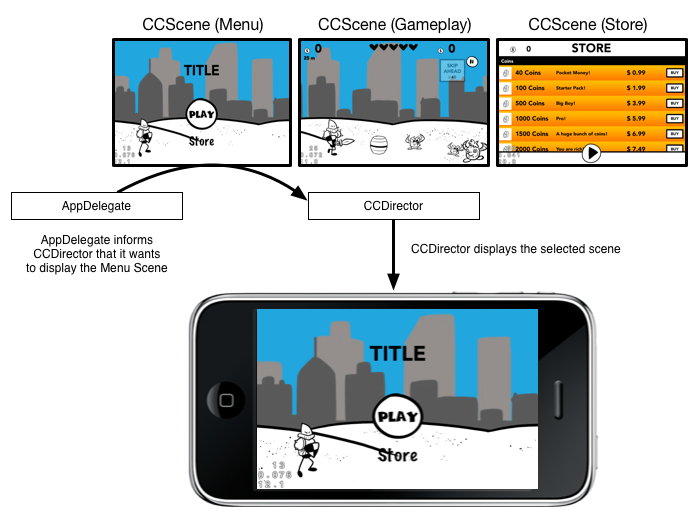
\includegraphics[width=400pt]{images/scenegraph.png}     
		\caption{\textit{Scene graph} in \cocos{}.}
		%\label{labelstruct} 
\end{figure}
 
The diagram represents three different scenes of which each contains
multiple nodes (all buttons, characters, etc. you can see). There are a couple
of takeaways from this diagram:

\begin{itemize}
  \item \textbf{CCDirector} is the highest instance in \cocos{}. It will control
  which scene is presented. You can tell CCDirector to present your main menu,
  your gameplay scene or your highscore scene. CCDirector will allow you to
  present one scene at a time.
  \item \textbf{CCScenes} are used to build a logical group of objects. In
  \cocos{} this almost always means - one scene represents one screen. You will
  have scenes for menues, leaderboards, gameplay, etc. Scenes itself don't have
  a representation, their sole goal is to group CCNodes.
  \item \textbf{CCNodes}. Simply speaking anything that is visible in \cocos{}
  is a subclass of CCNode. We will get to know a diverse range of CCNode
  subclasses very soon, including UI Elements and Sprites\footnote{Sprite
  basically is the game developer word for an image}.
\end{itemize}

The games we write in \cocos{} consist of different scenes. We define the
structure of our game by telling the CCDirector when which scene shall be
presented (menu first, then gameplay, then leaderboard). We create the content
of our scenes using CCNodes.

A CCNode can again contain other CCNodes. We are speaking of a scne graph when
we refer to the strucutre of our CCNodes.

\section{CCNodes in \cocos{} 3.0}
We just learned: \textit{Every visible object in \cocos{} is a subclass of
CCNode}. These are the CCNode subclasses you should know for now:

\begin{description}
  \item[CCSprite] Represents an image or an animated image. Used for characters,
  enemies, etc. in your gameplay.
  \item[CCAnimatedSprite] A convinience class that allows to create animated
  Sprites in just a few lines of code.
  \item[CCNodeColor] A plain colored node.
  \item[CCLabelTTF] A node than represent text in any TTF font.
  \item[CCButton] A interactive node that allows to respond to touch input
  easily.
  \item[CCLayoutBox] A unvisible node that layouts its children.
\end{description}

\section{Let's code}
The easiest way to prove, that \cocos{} is an easy-to-learn, powerful framework
is by starting to write some code. What you have learned so far is enough to
build a simple App with multiple scenes.

Here are the code snippets for the concepts we have already discussed:
\begin{lstlisting}[title=examples/introduction.clj]
[CCDirector sharedDirector]
basically, create a menu scene, create a gameplay scene, add a animated
character to the gameplayscene
\end{lstlisting} 


\begin{error}
Having problems installing \cocos{}? Visit\ldots.
\end{error}